\section{Support Vector Machine}
\script{337}
SVM lösen Klassifizierungsprobleme und haben den Vorteil, dass nur wenige Trainigsdaten benötigt werden. 
\begin{center}
	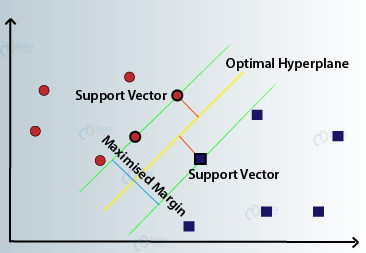
\includegraphics[width=0.7\columnwidth]{Images/svm_details}
\end{center}

Links ein Maximal margin classifier. Rechts ein Support Vector Classifier, links kann kein Support Vector Classifiert sein, weil Punkt 8 und 1 auf der falschen Seite sind.
\begin{center}
	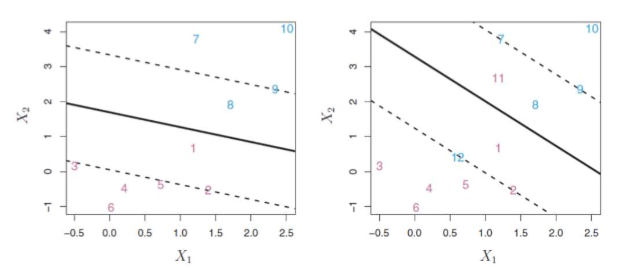
\includegraphics[width=\columnwidth]{Images/svm}
\end{center}

Mittels einem Parameter $C$, können diese Ränder gesteuert werden. Für $C=0$ resultiert ein Maximal margin classifiert. Bei $C\gt0$, können nicht mehr als $C$ Punkte auf der falschen Seite der Hyperplane sein -  $C$ kontrolliert den $Bias^2-Variance$ trad-off. Ein kleines $C$ gibt schmalle Margins, was für ein overfitting der Trainsdaten spricht, anders gibt ein grosses $C$ eine grössere Varianz.